\documentclass[t,usenames,dvipsnames]{beamer}
\usetheme{Copenhagen}
\setbeamertemplate{headline}{} % remove toc from headers
\beamertemplatenavigationsymbolsempty

\usepackage{amsmath, xcolor, tikz, pgfplots, array, bm}

\pgfplotsset{compat = newest}
\usetikzlibrary{arrows.meta, calc, decorations.pathreplacing}
\pgfplotsset{every axis/.append style = {axis lines = middle}}
\pgfplotsset{every tick label/.append style={font=\scriptsize}}
\everymath{\displaystyle}

\tikzstyle{input} = [circle, text centered, radius = 1cm, draw = black]
\tikzstyle{function} = [rectangle, text centered, minimum width = 2cm, minimum height = 1cm, draw = black]

\title{Exponential Functions}
\author{}
\date{}

\AtBeginSection[]
{
  \begin{frame}
    \frametitle{Objectives}
    \tableofcontents[currentsection]
  \end{frame}
}

\begin{document}

\begin{frame}
    \maketitle
\end{frame}

\section{Use exponential functions to solve problems}

\begin{frame}{Intro}
An \alert{exponential function} is a function in which each successive output value is obtained by {\color{violet}\textbf{multiplying}} the previous one by a constant value. \newline\\   \pause

One example of an exponential function is the {\color{blue}\textbf{doubling function}}
\[ f(x) = 2^x \]
\end{frame}

\begin{frame}{Doubling Function}
\begin{minipage}{0.6\textwidth}
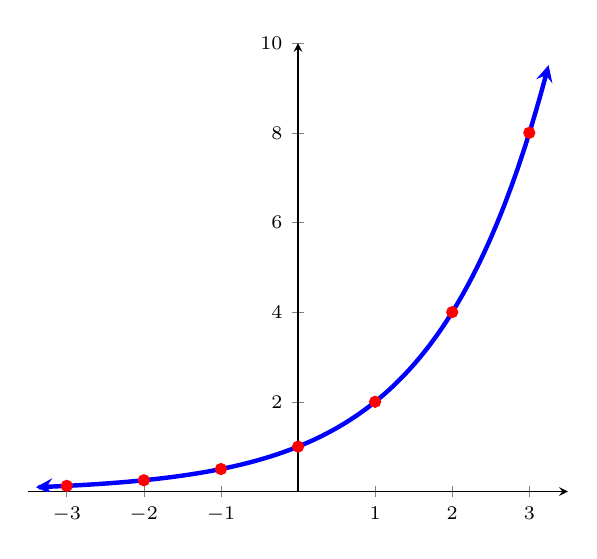
\begin{tikzpicture}
\begin{axis}[
xmin = -3.5, xmax = 3.5,
ymin = 0, ymax = 10
]
\addplot[color=blue, ultra thick, samples=200, smooth, domain=-3.4:3.25, <->, >=stealth] {2^x};
\addplot[color=red, mark = *, only marks] coordinates {(-3,0.125) (-2,0.25) (-1,0.5) (0,1) (1,2) (2,4) (3,8)};
\end{axis}
\end{tikzpicture}
\end{minipage}
\hspace{1cm}
\begin{minipage}{0.25\textwidth}
\setlength{\extrarowheight}{5pt}
\begin{tabular}{c|c}
    $x$ & $f(x)$ \\ \hline 
    $-3$ & $\tfrac{1}{8}$ \\[5pt]
    $-2$ & $\tfrac{1}{4}$ \\[5pt]
    $-1$ & $\tfrac{1}{2}$ \\[5pt]
    0   &   1   \\[5pt]
    1   &   2   \\[5pt]
    2   &   4   \\[5pt]
    3   &   8   
\end{tabular}
\end{minipage}
\end{frame}

\begin{frame}{End Behavior of the Doubling Function}
As the values of $x \to -\infty$, 
\[ 2^{\text{very big negative number}} \to 0 \] \pause
For instance,
\[ 2^{-50} \approx 0.0000000000000008882 \] \pause
\bigskip

As the values of $x \to \infty$,
\[ 2^{\text{very big positive number}} \to \infty \]    \pause
For instance,
\[ 2^{50} = 1,125,899,906,842,624\]
\end{frame}

\begin{frame}{Exponential Functions}
A function in the form $f(x) = b^x$ where $b$ is a fixed real number, $b > 0, b \neq 1$ is called an \textbf{exponential function of base $\bm{b}$}  \newline\\  \pause
\begin{minipage}{0.45\textwidth}
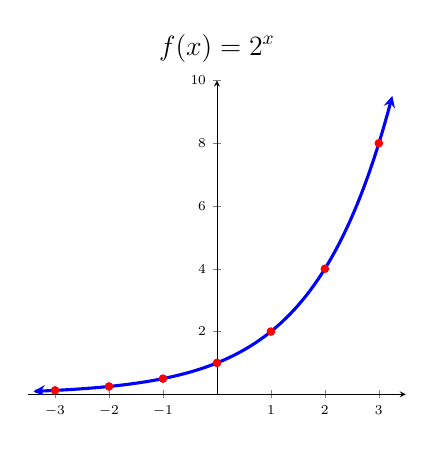
\begin{tikzpicture}[scale=0.7]
\begin{axis}[
xmin = -3.5, xmax = 3.5,
ymin = 0, ymax = 10,
title = {\Large $f(x)=2^x$}
]
\addplot[color=blue, ultra thick, samples=200, smooth, domain=-3.4:3.25, <->, >=stealth] {2^x};
\addplot[color=red, mark = *, only marks] coordinates {(-3,0.125) (-2,0.25) (-1,0.5) (0,1) (1,2) (2,4) (3,8)};
\end{axis}
\end{tikzpicture}
\end{minipage}
\hspace{0.5cm}
\begin{minipage}{0.45\textwidth}
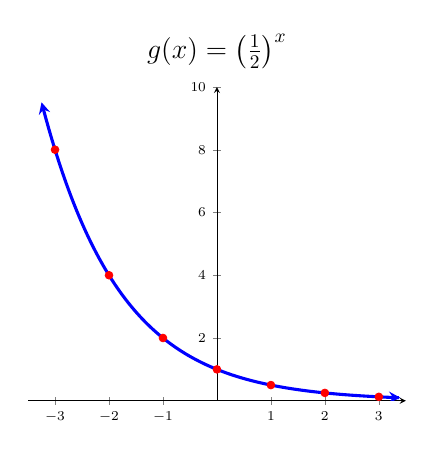
\begin{tikzpicture}[scale=0.7]
\begin{axis}[
xmin = -3.5, xmax = 3.5,
ymin = 0, ymax = 10,
title = {\Large $g(x) = \left(\frac{1}{2}\right)^x$}
]
\addplot[color=blue, ultra thick, samples=200, smooth, domain=-3.25:3.4, <->, >=stealth] {2^-x};
\addplot[color=red, mark = *, only marks] coordinates {(-3,8) (-2,4) (-1,2) (0,1) (1,0.5) (2,0.25) (3,0.125)};
\end{axis}
\end{tikzpicture}
\end{minipage}
\end{frame}

\begin{frame}{Properties of Exponential Functions}
For $f(x) = b^x$:   \newline\\
\begin{itemize}
    \item Domain is $(-\infty, \infty)$ and the range is $[0,\infty)$ \newline\\ \pause
    \item $(0,1)$ is on the graph of $f$ and $y=0$ is a horizontal asymptote. \newline\\ \pause
    \item $f$ is one-to-one (has an inverse), continuous, and smooth.
\end{itemize}
\end{frame}

\begin{frame}{Properties of Exponential Functions}
For $f(x) = b^x$ when $b > 1$:  \newline\\
\begin{itemize}
    \item $f$ is always increasing  \newline\\  \pause
    \item $\lim_{x\to -\infty} = 0 \quad \text{and} \quad \lim_{x\to \infty} = \infty$ \newline\\ \pause
    \item The graph of $f$ resembles
\end{itemize}
\begin{center}
    \begin{tikzpicture}[scale=0.5]
    \begin{axis}[
    xmin = -2, xmax = 2,
    ymin = 0, ymax = 4.5,
    ticks=none
    ]
    \addplot[blue, very thick, samples=200, smooth] {2^x};
    \end{axis}
    \end{tikzpicture}
\end{center}
\end{frame}

\begin{frame}{Properties of Exponential Functions}
For $f(x) = b^x$ when $0 < b < 1$:  \newline\\
\begin{itemize}
    \item $f$ is always decreasing  \newline\\  \pause
    \item $\lim_{x\to -\infty} = \infty \quad \text{and} \quad \lim_{x\to \infty} = 0$ \newline\\ \pause
    \item The graph of $f$ resembles
\end{itemize}
\begin{center}
    \begin{tikzpicture}[scale=0.5]
    \begin{axis}[
    xmin = -2, xmax = 2,
    ymin = 0, ymax = 4.5,
    ticks=none
    ]
    \addplot[blue, very thick, samples=200, smooth] {2^-x};
    \end{axis}
    \end{tikzpicture}
\end{center}
\end{frame}

\begin{frame}{Special Bases}
Of all possible bases for exponential functions, the 2 that occur most are base 10 (\alert{common base}) and irrational base $e \approx 2.718$ (\alert{natural base}). \newline\\

\[ e = \lim_{x \to \infty} \left(1 + \frac{1}{x}\right)^x \]
\end{frame}

\begin{frame}{Example 1}
The value of a car can be modeled by $V(x) = 25\left(\frac{4}{5}\right)^x$, where $x \geq 0$ is the age of the car in years and $V(x)$ is the value in thousands of dollars.    \newline\\
(a) \quad Find and interpret $V(0)$   \newline\\  \pause
$V(0)$ is the value of the car (in thousands of dollars) when it's brand new. 
\begin{align*}
    \onslide<3->{V(0) &= 25\left(\frac{4}{5}\right)^0} \\[10pt]
    \onslide<4->{&= 25} 
\end{align*}

\onslide<5->{Brand new, the car is valued at \$25,000.}
\end{frame}

\begin{frame}{Example 1}
(b) \quad Find the parent function and describe the function $V(x) = 25\left(\frac{4}{5}\right)^x$ using transformations.    \newline\\  \pause

Parent function is $f(x) = \left(\frac{4}{5}\right)^x$  \newline\\   \pause
$V(x) = 25\left(\frac{4}{5}\right)^x$ is a vertical stretch by a factor of 25.
\end{frame}

\begin{frame}{Example 1}
(c) \quad Find and interpret the horizontal asymptote of the graph of $V(x)$. \newline\\  \pause

Horizontal asymptote is $y = 0$. \newline\\ \pause
Over time, the value of the car will approach 0.
\end{frame}

\begin{frame}{Example 2}
According to Newton's Law of Cooling, the temperature of coffee $T$ (in degrees Fahrenheit) $t$ minutes after it is served can be modeled by
\[ T(t) = 70 + 90e^{-0.1t} \]
\bigskip
(a) \quad Find and interpret $T(0)$. 
\begin{align*}
    \onslide<2->{T(0) &= 70 + 90e^{-0.1(0)}} \\
    \onslide<3->{&= 160}
\end{align*}
\onslide<4->{The coffee was served at $160^\circ$F.}
\end{frame}

\begin{frame}{Example 2}
\[ T(t) = 70 + 90e^{-0.1t} \]

(b) \quad Find the parent funtion and describe the function $T(t)$ using transformations. \newline\\  \pause

Parent function is $f(t) = e^t$ \newline\\  \pause
$T(t)$ is the parent function with the following transformations:   \newline\\
\begin{itemize}
    \item Reflection across $y$-axis (multiplying $t$ by $-1$) \pause
    \item Horizontal stretch by factor of 10 (multiplying $t$ by 0.1) \pause
    \item Vertical stretch by factor of 90 \pause
    \item Shift up 70 degrees Fahrenheit
\end{itemize}
\end{frame}

\begin{frame}{Example 2}
(c) \quad Find and interpret the horizontal asymptote of the graph.   \newline\\ \pause

Horizontal asymptote = 70   \newline\\  \pause

Over time, the coffee will cool to a temperature of $70^\circ$F.
\end{frame}

\end{document}
